%; whizzy chapter
% -initex iniptex -latex platex -format platex -bibtex jbibtex -fmt fmt
% 以上 whizzytex を使用する場合の設定。

%     Tokyo Debian Meeting resources
%     Copyright (C) 2011 Junichi Uekawa
%     Copyright (C) 2011 Nobuhiro Iwamatsu

%     This program is free software; you can redistribute it and/or modify
%     it under the terms of the GNU General Public License as published by
%     the Free Software Foundation; either version 2 of the License, or
%     (at your option) any later version.

%     This program is distributed in the hope that it will be useful,
%     but WITHOUT ANY WARRANTY; without even the implied warranty of
%     MERCHANTABILITY or FITNESS FOR A PARTICULAR PURPOSE.  See the
%     GNU General Public License for more details.

%     You should have received a copy of the GNU General Public License
%     along with this program; if not, write to the Free Software
%     Foundation, Inc., 51 Franklin St, Fifth Floor, Boston, MA  02110-1301 USA

%  preview (shell-command (concat "evince " (replace-regexp-in-string "tex$" "pdf"(buffer-file-name)) "&"))
% 画像ファイルを処理するためにはebbを利用してboundingboxを作成。
%(shell-command "cd image201101; ebb *.png")

%%ここからヘッダ開始。

\documentclass[mingoth,a4paper]{jsarticle}
\usepackage{monthlyreport}

% 日付を定義する、毎月変わります。
\newcommand{\debmtgyear}{2011}
\newcommand{\debmtgmonth}{6}
\newcommand{\debmtgdate}{18}
% (+ (* (- 2011 2005) 12) 6 -1) started from zero
\newcommand{\debmtgnumber}{77}

\begin{document}

\begin{titlepage}
\thispagestyle{empty}
% タイトルページ:編集必要な部分は最初のマクロに飛ばすこと

\vspace*{-2cm}
第\debmtgnumber{}回 東京エリア Debian 勉強会資料\\
\hspace*{-2cm}
\includegraphics[width=210mm]{image201003/debsen.eps}\\
\hfill{}\debmtgyear{}年\debmtgmonth{}月\debmtgdate{}日

% ここはアップデートすること
\rotatebox{10}{\fontsize{32}{32} {\gt 特集1: DebianでXSLTを使ってみた}}

\rotatebox{10}{\fontsize{32}{32} {\gt 特集2: SphinxとDoxygenを使ってみた}}

\vspace*{-2cm}
\hfill{}
\includegraphics[height=6cm]{image200502/openlogo-nd.eps}
\end{titlepage}

\dancersection{Introduction}{上川 純一}

\begin{multicols}{2}
 

 今月のDebian勉強会へようこそ。これからDebianの世界にあしを踏み入れると
 いう方も、すでにどっぷりとつかっているという方も、月に一回Debianについ
 て語りませんか?

 Debian勉強会の目的は下記です。

 \begin{itemize}
 \item \underline{Debian Developer} (開発者)の育成。
 \item 日本語での「\underline{開発に関する情報}」を整理してまとめ、アップデートする。
 \item \underline{場}の提供。
 \begin{itemize}
  \item 普段ばらばらな場所にいる人々が face-to-face で出会える場を提供
	する。
  \item Debian のためになることを語る場を提供する。
  \item Debianについて語る場を提供する。
 \end{itemize}
 \end{itemize}		

 Debianの勉強会ということで究極的には参加者全員がDebian Packageをがりがり
 と作るスーパーハッカーになった姿を妄想しています。情報の共有・活用を通し
 て Debianの今後の能動的な展開への土台として、「場」としての空間を提供す
 るのが目的です。

\end{multicols}

\newpage

\begin{minipage}[b]{0.2\hsize}
 \definecolor{titleback}{gray}{0.9}
 \colorbox{titleback}{\rotatebox{90}{\fontsize{80}{80} {\gt デビアン勉強会} }}
\end{minipage}
\begin{minipage}[b]{0.8\hsize}
\hrule
\vspace{2mm}
\hrule
\begin{multicols}{2}
\tableofcontents
\end{multicols}
\vspace{2mm}
\hrule
\end{minipage}

\dancersection{事前課題}{岩松 信洋}

今回の事前課題は以下です:
\begin{enumerate}
 \item 最近Debianで自分がやったことや興味のあることを教えてください。
\end{enumerate}
この課題に対して提出いただいた内容は以下です。
\begin{multicols}{2}
{\small
 
\begin{prework}{ やまだ }

最近新しいカーネルを自分でビルドすることが再び
増えてきたので、その周りでごそごそやってます。
\begin{enumerate}
\item gitでタグを打って
\item そのタグをバージョンにして
\item ビルドして
\item テストVMに導入して
\item ついでに配布サーバに設置
\end{enumerate}

の自動化とかやりました。

興味というか次に調べたいのは *-module-source な
カーネルモジュールパッケージの作り方とかDKMSの使い方。
普通のパッケージと違う点が多々ありそう。
\end{prework}

\begin{prework}{ 野首 }

ホームのMHフォルダを外から見れるようuw-imapdを入れました。インストールし
 てdebconfに答えるだけでSSL readyなimap環境になりました。
\end{prework}

\begin{prework}{ MATOHARA }

2010年11月の勉強会資料を見ながらnilfs2 をバックアップディスクに設定して
 みました.
リサイズ機能も来たようなので試してみたいです.
- [PATCH 0/4] nilfs2 resize support -- Linux NILFS Development
\url{http://www.spinics.net/lists/linux-nilfs/msg00869.html}
\end{prework}

\begin{prework}{ hattorin }

バングラデシュでDebianインストールして、ネットワークの監視系ツールをいろ
 いろとセットアップしてきました。今はDebian on SqueezeでTokyoTyrantの
 KeyValueを使い、特定の問題を早く計算するためにネットワークを使って計算
 を早くするような仕組み作りをしています。
\end{prework}

\begin{prework}{ キタハラ }

実家でプリンタの設定したり、
スキャナーの設定に失敗してました。

\end{prework}

\begin{prework}{ koedoyoshida }

最近Debianで自分がやったこと
\begin{itemize}
\item ようやく、メイン環境をSqueezeにupdate
wide-dhcpがupdateできずにはまったが、下記を見て解決。
\url{http://www.flcl.org/~takasugi/tdiary-org/?date=20061023}
\item OSC仙台に参加、出展。
\end{itemize}


\end{prework}

\begin{prework}{ emasaka }

sidでちょっとはまったとこについて、GitHubでupstreamに簡単なパッチをpull
 requestしたら、そのバージョンが数日後にsidに降りてきました。
\end{prework}

\begin{prework}{ dictoss(杉本 典充) }

最近やっていることはkfreebsdを常用していること、Debianを開発環境として
 gtkアプリを試作していること。
今後はkfreebsdでIS03を使ってテザリング、klinuxよりkfreebsdの方がおすすめ
 といえる有利分野を見つけることをやりたい。
\end{prework}

\begin{prework}{ なかおけいすけ }

興味があること:DebianLive
最近ネカフェで一夜を明かしたのですが、ネカフェのPCにコンパイラが入ってな
 くて困ったので、USBやSDカードにインストールしたDebianを持ち歩いていると
 ハッピーになれるのではないかと。
\end{prework}

\begin{prework}{ 吉野(yy\_y\_ja\_jp) }

バグレポートとDDTSS/DDTPぐらいでしょうか.
\end{prework}

\begin{prework}{ henrich }

いくつかパッケージやメッセージをルーティンの更新しました。

\end{prework}

\begin{prework}{ Osamu MATSUMOTO }

\begin{itemize}
\item インフラ,サーバ管理の自動化\\
 自動インストール,構成管理,コンフィグ投入, 監視のまでを
 ラフに綺麗に繋ぎたい。Debian的な良い組み合わせあったら教えてください。
 (cobbler+ puppet/cfengine+ nagios + なんかwebcgi的な)
\end{itemize}

\end{prework}

\begin{prework}{ まえだこうへい }
\begin{itemize}
\item *diagシリーズ(http://blockdiag.com/)のdebパッケージ化中。
\item さくらのVPSを先月契約して、lxc \& Squeezeで開発\&検証環境に。
\item あらきさんメンテナンスのDebianのAMI使ってAWSでごにょごにょと。
\end{itemize}
\end{prework}

\begin{prework}{ yamamoto }

\begin{itemize}
\item 最近Debianで自分がやったこと\\
ポチポチと公式パッケージのリビルドをしました。
\item 興味のあること\\
移植。
\end{itemize}

\end{prework}

\begin{prework}{ 岩松 信洋 }

\begin{itemize}
\item SH4 buildd のメンテ。
\item libpng15 の experimental へのアップロードとtransition作業。
\item スポンサーのパッケージチェック、アップロードなど。
\end{itemize}

\end{prework}

\begin{prework}{ 野島 貴英 }

\begin{itemize}

\item pythonでgnome-notifyめがけて再生中のデータのメタデータ送る「できるだ
 け簡単にできる」totemのプラグイン書いてみた。
 \url{http://d.hatena.ne.jp/nozzy123nozzy/20110502/1304322969}
\item sidのalsa-lib,alsa-utils,alsa-driverの解析中。
(bluetoothヘッドフォン出力相手に、alsaのみで、演奏中の音をcaptureしたい
 し、音が出る複数のアプリの音をmixして出力したいっ)
\item sidのlinux-image-2.6.39-2-686-paeにて、multi-stateなusb装置にejectコ
 マンド発行すると高い確率でOopsする件のデバッグを誰かがパッチ出すまでや
 り中。(いったい誰だ、dptぶっ壊すのは...)

\end{itemize}

\end{prework}

\begin{prework}{ 上川純一 }
\begin{itemize}
\item xslt のツールチェインをいろいろといじってみたり。
\item Javascript のコードを書いてみたり。
\end{itemize}
\end{prework}

}
\end{multicols}

\dancersection{最近のDebian関連のミーティング報告}{岩松 信洋}
\subsection{東京エリアDebian勉強会76回目報告}

東京エリアDebian勉強会76回目は新大久保駅
の近くにある戸山生涯学習館で行いました。
上川さんが apache2 のモジュールの作成についてお話しし、
Debian のapache2モジュール作成のはまりどこについて盛り上がりました。\\
Nifty さんがNifty Cloud に Debian 
使えるようにするということで、どのようなイメージにしたらいいのか、どのようなバックエンドが必要なのか議論しました。NiftyさんでそろそろDebianが使えるようになっていると思います(たぶん)。
岩松が Debian での m68k 開発についての状況と方法を話しました。Debian では実機はあまり使われておらず、Aranymというエミュレータ上で開発を行っているとのこと。Debian で m68k が再度リリースされる日はくるのか楽しみです。
山本さんがppc64ポーティングについて報告しました。前回の宿題では powerpcspe とのベンチマークを取ってきて、ppc64と比べてどのようなメリットデメリットがあるのかを見てみようということでしたが、なぜかppcとのベンチを取ってきたので再度宿題になりました。パッケージは揃っているので家にppc64マシンが眠っている人は試してみてはいかがでしょうか。


% (query-replace-regexp "<.*?>" "")
% (query-replace-regexp "^[	 ]\+" "")

\subsection{OSC 2011 Hokkaido 出張Debian勉強会報告}
2011年6月11日(土)に北海道札幌市でオープンソースカンファレンス2011北海道が開催されました。

Debian勉強会ではタイトル「Debian 6.0(squeeze) \& Debian Update」として佐々木洋平さんがセッションを行いました。
セッションには14名が参加し、質問ではバグ報告の手順を確認する質問が出されました。


GPGキーサインパーティの参加者はコーディネーターを含めて3名であり、北海道の方々へGPGキーの啓蒙活動を引き続き行っていく必要がありそうです。

\begin{center}
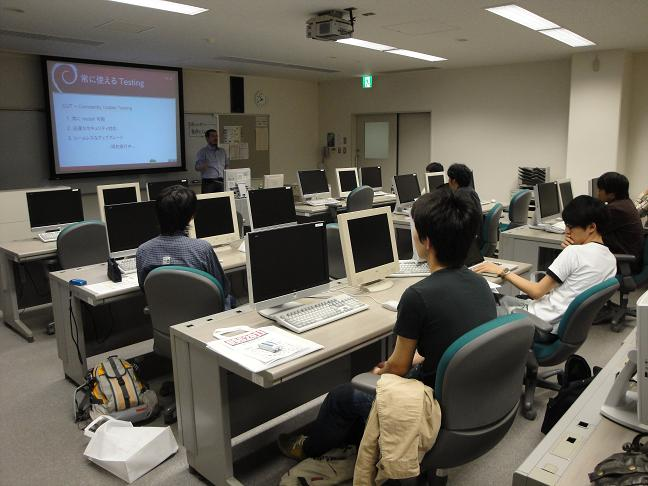
\includegraphics[width=10cm]{image201106/osc11do.jpg}
\end{center}

\subsection{OSC 2011 Sendai 出張Debian勉強会報告}
2011年5月21日(土)に宮城県仙台市でオープンソースカンファレンス2011仙台が開催されました。

Debian勉強会では吉田@板橋が展示で出展しました。
\begin{enumerate}
\item「東京エリアDebian勉強会/関西Debian勉強会」の紹介
\item「あんどきゅめんてっどでびあん(Debian勉強会資料のサマリ)」の展示、販売
\item「Debian Squeezeの展示」具体的には「Debian GNU/kFreeBSD」の展示
\end{enumerate}
主に上記をおこないました。
メインホール入り口正面という配置にも恵まれ、多くの方に立ち寄って頂きました。

\begin{center}
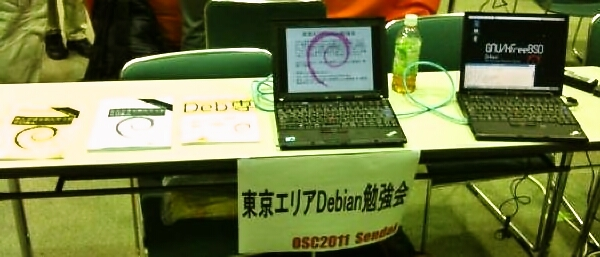
\includegraphics[width=10cm]{image201106/oscsendai.jpg}
\end{center}

\dancersection{Debian Trivia Quiz}{岩松 信洋}

ところで、みなさん Debian 関連の話題においついていますか?Debian関連の話
題はメーリングリストをよんでいると追跡できます。ただよんでいるだけではは
りあいがないので、理解度のテストをします。特に一人だけでは意味がわからな
いところもあるかも知れません。みんなで一緒に読んでみましょう。

今回の出題範囲は\url{debian-devel-announce@lists.debian.org} や \url{debian-devel@lists.debian.org}に投稿された
内容とDebian Project Newsからです。

\begin{multicols}{2}
 %; whizzy-master ../debianmeetingresume201101.tex
% $B0J>e$N@_Dj$r$7$F$$$k$?$a!"$3$N%U%!%$%k$G(B M-x whizzytex $B$9$k$H!"(Bwhizzytex$B$,MxMQ$G$-$^$9!#(B
%
% $B$A$J$_$K!"%/%$%:$OJL%V%i%s%A$G:n@.$7!"$N$A$K%^!<%8$7$^$9!#5U$K%^!<%8$7(B
% $B$J$$$h$&$K$7$^$7$g$&!#(B
% (shell-command "git checkout quiz-prepare")

\santaku
{alioth.debian.org$B$,(B2$BBf$KJ,$+$l$^$7$?!#$=$N%5!<%PL>$O!)(B}
{vasks.debian.org $B$H(B wagner.debian.org}
{volks.debian.org $B$H(B don.debian.org}
{dennys.debian.org $B$H(B gusto.debian.org}
{A}
{$B$[$+$O%U%!%_%l%9$NL>A0(B}

\santaku
{$B8=:_9T$o$l$F$$$k(BPerl transition $B$N(BPerl$B%P!<%8%g%s$O!)(B}
{5.12}
{5.13}
{5.14}
{A}
{5.14$B$O$^$@(Bexperimental$B$G$9!#(B}

\santaku
{$B%W%i%$%^%j%_%i!<%5!<%P$,?7$7$/DI2C$5$l$?9q$O!)(B}
{$B%A%e%K%8%"(B}
{$BCf9q(B}
{$B%^%@%,%9%+%k(B}
{B}
{$B%A%e%K%8%"$H%^%@%+%9%+%k$O%_%i!<!#%W%i%$%^%j$G$O$J$$!#(B}

\end{multicols}

%-------------------------------------------------------------------------------
\dancersection{Debian JP 定例会議処理系にXSLTを使ってみた}{上川純一}
%-------------------------------------------------------------------------------
\index{xsltproc}

\subsection{背景}

Debian勉強会の企画会議はIRCを中心として2006年に開始し、Debian JP の定例会
議として今も続いています。当初は決定事項などについてテキストファイルでま
とめるという形をとっていました。IRCでより効率よく議論する方法を模索した結
果、議論しながら議事録を編集するというスタイルが確立し、それを支援するた
めのツールを整備しました。

議事録のソースは議長がXMLで記述して、議論の最中は非同期にJavascriptで内
容が更新されるHTMLファイルを利用します(世間一般ではAJAX的とでもよぶよう
です)。

IRCでの定例会議の議論の前と後には議事案と議事録をメーリングリストにおくっ
ています。メーリングリストにメールでなげる際には、テキストフォーマットに
して送っています。

あと、現在用途がないですが、\LaTeX 経由でPDF形式での出力などもサポートし
ています。

現在の実装は歴史的な経緯によりXMLの処理系は dancer-xml ライブラリと
boostを利用したC++のプログラムになっています。
dancer-xml\cite{dancer-xml} は10年前に若気のいたりで実装したXML風文書のパー
サーです。一部エンティティーまわりなど真面目に実装していない部分があるた
め、適切な処理がなされていないことがありますが、僕の好みに空白文字処理は
チューニングされており快適です。

今回の挑戦は、独自C++コードベースをXSLTにのせ替えてみるという挑戦です。

\begin{figure}[ht]
 \begin{center}
  \includegraphics[width=0.5\hsize]{image201106/ircsystem.eps}
 \end{center}
\label{fig:ircsystem-general}\caption{IRC 会議システムのデータ形式の概要}
\end{figure}

\subsection{XSLTってどんな言語?}

XSLTはXMLで記述するXML処理言語です。

XSLT規格には1999年に策定されたXSLT 1.0 と、2007年ごろのXSLT 2.0があります。
今回は実装が十分枯れていると思われる XSLT 1.0 の処理系を採用しました。
XSLT2.0のDebianで利用できる実装としては libsaxonb-javaがある
ようですが、今回は調査していません。

プログラムを書くときにすべき文書としては、XSLT自体の1999年に策定された規
格\cite{xslt1999}と、XSLTの中で記述できるXPATHの規格\cite{xpath1999}を参
照するとよいでしょう。

XSLTだけではあまり高度なプログラミングはできないんじゃないかと思われるか
もしれませんが、関数型言語として十分な機能を提供できる力はあるようです
\cite{fxslt2003}。

\subsection{Debian で利用可能な XSLT処理系}

Debianで幅広く使われていて安定しているとおもわれるのと、簡単に利用できる
という理由で処理系として xsltproc を採用しました。

Debian での xsltproc のインストールは簡単
\begin{commandline}
$ apt-get install xsltproc
\end{commandline}
%$

コマンドラインで以下のように実行すると標準出力に処理済みXMLが出力されます。

\begin{commandline}
$ xsltproc [スタイルシート] [処理するXMLファイル]
\end{commandline}
%$

\subsection{具体例:HTML}

それでは、HTML出力の場合を見てみましょう。
\url{meetinglog:html.xsl}です。
XML文書からHTML文書を生成するにはそれなりに便利な言語です。

前半のコードをそのまま掲載します。
これは、XMLドキュメント全体にマッチするルールを記述しはじめるまでの部分
です。
XML名前空間として、デフォルトをHTML、xslをxsltの名前空間に割り当てていま
す。

xml:output で出力形式をHTMLと指定することでXMLヘッダが出力されずに便利で
す。

\begin{commandline}
<?xml version="1.0"?>
<!DOCTYPE xsl:stylesheet>
<xsl:stylesheet version="1.0"
  xmlns:xsl="http://www.w3.org/1999/XSL/Transform"
  xmlns="http://www.w3.org/1999/xhtml">
  <xsl:output method="html" />
  <xsl:template match="/">
    <html>
      <head>
\end{commandline}

他にXSLTの特徴的なところは、value-of で値をとってきています。XPATH
の書式で指定していますが、
\begin{commandline}
	<h1><xsl:value-of select="meetinglog/head/title"/></h1>
\end{commandline}

は、XML文書の以下のようなエレメントに入っている値を抽出します。
\begin{commandline}
 <meetinglog>
   <head>
     <title>タイトル</title>
   </head>
 </meetinglog> 
\end{commandline}

議事録の場合のメインループは、各議事に対しての処理です。
xslのxsl:for-eachをつかい、XMLのエレメントノードの数だけループします。
HTMLタグはそのまま出力されますが、もしHTMLのアトリビュートなどをXSLTで生
成したい場合は、xsl:element を使ってエレメントを生成します。

position()関数は現在のエレメント番号をくれるのでこういう場合に便利です。

\begin{commandline}
           <xsl:for-each select="meetinglog/body">
	      <tr>
		<th>
		  <xsl:element name="a">
		    <xsl:attribute name="href">#gian<xsl:value-of select="position()" /></xsl:attribute>
		  </xsl:element>
		  議案<xsl:value-of select="position()" />
		</th>
		<td class="bodytitle">
		  <xsl:value-of select="./title" />
		</td>
 ....
 </xsl:for-each> 
\end{commandline}

\subsection{具体例:Text出力}

Text出力の場合もみてみましょう。
\url{meetinglog:txt.xsl}
テキスト出力をしようとしはじめると若干苦しくなってきます。できないわけで
はないのですが、空白文字の処理のルールを僕がいまいち理解できていないのと、
コードがそのままテンプレートとして出力されるのでインデンテーションが適切
にできないのがつらいところです。

xsl:output で出力がテキスト形式であると指定するとXMLヘッダが出力されず便
利です。

ヘッダ部分で、毎回 xsl:text で改行などを入力するのが面倒なので、ENTITY を
定義して省略できるようにしています。この記法が正しいのかどうかは不明です。

\begin{commandline}
<?xml version="1.0"?>
<!DOCTYPE xsl:stylesheet [
<!ENTITY space  "<xsl:text xmlns:xsl='http://www.w3.org/1999/XSL/Transform'> </xsl:text>">
<!ENTITY indent "<xsl:text xmlns:xsl='http://www.w3.org/1999/XSL/Transform'>  </xsl:text>">
<!ENTITY cr     "<xsl:text xmlns:xsl='http://www.w3.org/1999/XSL/Transform'>
</xsl:text>">]>
  <xsl:stylesheet version="1.0"
    xmlns:xsl="http://www.w3.org/1999/XSL/Transform"
    xmlns="http://www.w3.org/1999/xhtml">
  <xsl:output method="text" />
  <xsl:template match="/">
    <xsl:text>-----------------------------------------------------------------------
概要
-----------------------------------------------------------------------
\end{commandline}

本文のコアとなる本文の内容ですが、読めたものではないです。
悩んだところとしては、文章が空白かどうかチェックするのに
string-length(normalize-space())をつかっていて、それがいまいちただしいの
かどうか自信がないところ。

\begin{commandline}
    <xsl:for-each select="meetinglog/body">
-----------------------------------------------------------------------
[<xsl:value-of select="position()" />.&space;<xsl:value-of select="./title" />]
-----------------------------------------------------------------------

目的: &cr;<xsl:value-of select="./aim" />&cr;
&cr;<xsl:if
 test="string-length(normalize-space(./previous))>1"
 >前回までの経緯:&cr;<xsl:value-of select="./previous"
 disable-output-escaping="yes" />&cr;&cr;</xsl:if>
<xsl:if test="string-length(normalize-space(./discussed))>1"
 >議論:&cr;<xsl:value-of select="./discussed"
 disable-output-escaping="yes" />&cr;&cr;&cr;
</xsl:if>
</xsl:for-each>
\end{commandline}

残念ながらC++で実装していた文字をメールの70文字幅くらいにきれいにまとめ
るというロジックが欠落しています。めんどくさすぎる。

\subsection{具体例:\LaTeX}

\LaTeX 出力をみてみましょう。
\url{meetinglog:latex.xsl}

ヘッダ部分はどうぜ\LaTeX{}のヘッダなのと何度もでてきているのでメインループ
だけ。
\begin{commandline}
    <xsl:for-each select="meetinglog/body">

      \discussion{<xsl:value-of select="./title" />}{<xsl:value-of
 select="./aim" />}{<xsl:value-of
 select="translate(./previous,'#&amp;','--')"
 disable-output-escaping="yes" />}{<xsl:value-of
 select="translate(./discussed,'#&amp;','--')"
 disable-output-escaping="yes" />}
    </xsl:for-each>
\end{commandline}

個人的な感想ですが、自分で書いておきながら後で読み返す気力が沸きません。

現在実装できていない点として、\LaTeX{}で使えない文字列\verb!#<>&!などの文
字列のエスケープがあります。今はハイフンに変更してお茶を濁しています。

XPATHには文字列置換のためのtransform()関数がありますが、一文字を一文字に置換
することしかできません。今回行いたいのは一文字を複数文字に置換することな
のでそれでは機能が不十分です。

\subsection{仮の定量的な比較}

現状すべての機能をおきかえているわけではないので、妥当な比較ではないです
が、C++の処理とXSLTのコードの比較をしてみると
(\ref{tab:xsltcxximplementationdiff})、
XSLTのほうが行数は少ないことがわかります。

\begin{table}[ht]
 \caption{lines of code for each implementation}
 \label{tab:xsltcxximplementationdiff}
\begin{center}
  \begin{tabular}{|c|c|c|}
 \hline
 & c++ & xslt \\
 \hline
 txt & 151 & 53\\
 html & 157 & 99 \\
 latex(PDF) & 158 & 87 \\
 \hline
 \end{tabular}
\end{center}
\end{table}

\subsection{結論}

XSLTを使うことでメンテナンスする行数は少なくなります。しかし、XPATH /
XSLT により提供されている機能が制限されているため、その中で実現しにくい
機能についてはがんばるか提供を諦めるのか、難しい判断を迫られます。

\begin{thebibliography}{0}
 \bibitem{fxslt2003} Dimitre Novatchev, ``Functional programming in XSLT
	 using the FXSL library,'' Extreme Markup Languages 2003.
 \bibitem{xslt1999} James Clark, ``XSL Transformations (XSLT)
	 Version 1.0,'' W3C Recommendation 16 November 1999.
	 \url{http://www.w3.org/TR/xslt}
 \bibitem{xpath1999} James Clark, Steve DeRose, ``XML Path Language
	 (XPath) Version 1.0,'' W3C Recommendation 16 November 1999.
	 \url{http://www.w3.org/TR/xpath/}
 \bibitem{dancer-xml} Junichi Uekawa, ``dancer-xml - Simple
	 non-comformant XML parsing library,'' 2000.
	 \url{http://www.netfort.gr.jp/~dancer/software/dancer-xml.html}
\end{thebibliography}


%-------------------------------------------------------------------------------
\dancersection{DebianでSphinxとDoxygenを使ってみた}{まえだこうへい}
%-------------------------------------------------------------------------------
\index{sphinx}
\index{doxygen}

\subsection{最近の流行りのようです}

Python関連のプロジェクトやエンジニアを中心に最近流行っているようです。
Sphinx-Users.jpのサイトを見る\footnote{\url{http://sphinx-users.jp/example.html}}と、
2011年6月現在、Sphinxのデフォルトテーマだけでなく、カスタムテーマやオリジナルテー
マを使った、50弱の日本語のサイトが紹介されています。

\subsubsection{reSTとSphinxの概要}

SphinxはreST(reStructuredText)という軽量マークアップ言語で書いたソースを
様々なフォーマットのドキュメントに変換・生成するためのツールです。
出力可能なフォーマットには、HTML、 \LaTeX 、PDF、ePub、man、平文テキスト、JSONなどがあります。

\subsubsection{reSTのサンプル}

試しに、東京エリアDebian勉強会のページをreSTで書くとこんな感じになります。

\begin{commandline}
========================
 東京エリアDebian勉強会
========================


背景
====

2005年当初、東京近辺で、類似の勉強会は存在していませんでした。
Debian について語る場所を提供するため、 Debian 勉強会を開催します。 
この勉強会では毎回事前課題を設定しています。
その課題を提出することが参加の条件です。 
参加する方は宴会の都合もありますので、事前に登録してください。 
また、当日はDebianについての知識に関した簡単な試験を実施するので、
勉強会の会場には筆記用具を持参ください。

現在、 Debian 勉強会は
`Debian JP Project <http://www.debian.or.jp/>`_
のメンバーが Debian JP の公式なイベントとして運営しています。

次回の勉強会
============

* `2011年6月勉強会(第77回東京エリアDebian勉強会) <2011-06.html>`_
* `第48回関西Debian勉強会 <http://wiki.debian.org/KansaiDebianMeeting20110626>`_
* `毎週開催のハックカフェ <hackcafe.html>`_
(snip)
\end{commandline}

具体的な書式については、Sphinx-Users.jpのドキュメント\footnote{\url{http://sphinx-users.jp/doc.html}}を参照してください。

\subsection{Sphinxを使うきっかけ}

graphvizのdot言語と似た書式でブロック図を生成できるblockdiagシリーズ
\footnote{\url{http://blockdiag.com/}}というpythonで書かれたツールがあります。
最近、岩松さんにスポンサーをお願いして、これらのDebianパッケージ化を行っ
ています。これらのSphinx拡張機能(spyhinxcontrib-blockdiagなど)を使うと、
Sphinxで生成するドキュメントの中にブロック図を埋め込むことができます。
このblockdiagシリーズが便利なので、Sphinxを使いだしたようなものです。

また、仕事では基本的にMS Office、とくにExcelやPowerPointでの文書作成がほ
とんどなのですが、今期の最初に「もうMS Officeなんてでやってられっかー、
Sphinxで作ろうぜ!」と、プロジェクト内で提案して使い始めました。私個人で
作る分には \LaTeX でも良いのですが、他の二人はWindowsしか普段触ったことがな
い上、文書と言えば上述のとおり、ExcelかPowerPoint、という状態です。まっ
たく使ったことがない人に \LaTeX 文書を作成させるのは敷居が高すぎます。しか
し、reST \& Sphinxなら割と簡単に入門できる上、Windowsとの共同作業の環境
を整えるのもメンドイけど( \LaTeX 環境を整えるよりも)楽だった、という経緯です。\footnote{Windowsは改めてマンドイと思いました。\url{http://d.hatena.ne.jp/mkouhei/20110521/1305905297}}

\subsection{Debianで使ってみる}

試しに先ほどの東京エリアDebian勉強会のホームページをreSTで書いたものをSphinxで管理してみましょう。

まずはpython-sphinxパッケージをインストールしておきます。
\begin{commandline}
$ sudo apt-get install python-sphinx
\end{commandline}

emacsを使う場合は、python-docutilsパッケージをインストールしておけば、拡張子がrstかrestの場合、rst.elによって自動的にReSTモードになります。

\begin{commandline}
$ sudo apt-get install python-docutils
\end{commandline}

Sphinxプロジェクトを作ります。プロジェクト用のディレクトリを作ります。

\begin{commandline}
$ mkdir tokyodebian
$ cd tokyodebian
\end{commandline}

作成したディレクトリに移動して、\texttt{sphinx-quickstart}コマンドを実行
します。
\begin{commandline}
$ sphinx-quickstart 
\end{commandline}

このコマンドを実行すると対話形式で聞かれます。htmlを生成するので、
Project Name, Author name(s), Project Version以外はデフォルトのまま
(Enterを押下)で良いでしょう。(表\ref{tab:sphinx-quickstart})

\begin{table}[h]
{\scriptsize
 \caption{sphinx-quickstartの設定項目}\label{tab:sphinx-quickstart}
  \begin{tabular}{|l|c|c|}
    \hline
    設定項目 & デフォルト値 & 設定例 \\
    \hline
    Root path for the documentation & . & デフォルト \\
    Separate source and build directories (y/N) & n & デフォルト \\
    Name prefix for templates and static dir & \_ & デフォルト \\
    Project name: & & Tokyo Debian Meeting \\
    Author name(s) & & Debian JP Project \\
    Project version & & 1.0 \\
    Project release & 1.0 & デフォルト \\
    Source file suffix & .rst & デフォルト \\
    Name of your master document (without suffix) & index & デフォルト \\
    Do you want to use the epub builder (y/N) & n & デフォルト \\
    autodoc: automatically insert docstrings from modules (y/N) & n & デフォルト\\ 
    doctest: automatically test code snippets in doctest blocks (y/N) & n & デフォルト \\ 
    intersphinx: link between Sphinx documentation of different projects (y/N) & n & デフォルト \\
    todo: write ``todo'' entries that can be shown or hidden on build (y/N) & n & デフォルト \\ 
    coverage: checks for documentation coverage (y/N) & n & デフォルト\\
    pngmath: include math, rendered as PNG images (y/N) & n & デフォルト \\
    jsmath: include math, rendered in the browser by JSMath (y/N) & n & デフォルト \\
    ifconfig: conditional inclusion of content based on config values (y/N) & n & デフォルト\\
    viewcode: include links to the source code of documented Python objects (y/N) & n & デフォルト \\
    Create Makefile? (Y/n) & y & デフォルト \\
    Create Windows command file? (Y/n) & y & デフォルト \\
    \hline
  \end{tabular}
}
\end{table}

先ほどのtokyodebian.rst(および、hackcafe.rst, 2011-06.rst)をコピーします。
\begin{commandline}
$ cp -i ~/*.rst .
\end{commandline}

自動的に生成されるindex.rstにこれらを追記します。\footnote{拡張子不要です。}
\begin{commandline}
$ sensible-editor index.rst
---
.. Tokyo Debian Meeting documentation master file, created by
   sphinx-quickstart on Fri Jun 17 13:39:53 2011.
   You can adapt this file completely to your liking, but it should at least
   contain the root `toctree` directive.

Welcome to Tokyo Debian Meeting's documentation!
================================================

Contents:

.. toctree::
   :maxdepth: 2

   tokyodebian  ←追加
   hackcafe  ←追加
   2011-06  ←追加

Indices and tables
==================

* :ref:`genindex`
* :ref:`modindex`
* :ref:`search`

\end{commandline}

コンパイルします。
\begin{commandline}
$ make html
sphinx-build -b html -d _build/doctrees   . _build/html
Running Sphinx v1.0.7
loading pickled environment... done
building [html]: targets for 4 source files that are out of date
updating environment: 0 added, 4 changed, 0 removed
reading sources... [ 25%] 2011-06
reading sources... [ 50%] hackcafe
reading sources... [ 75%] index
reading sources... [100%] tokyodebian

looking for now-outdated files... none found
pickling environment... done
checking consistency... done
preparing documents... done
writing output... [ 25%] 2011-06
writing output... [ 50%] hackcafe
writing output... [ 75%] index
writing output... [100%] tokyodebian

writing additional files... genindex search
copying static files... done
dumping search index... done
dumping object inventory... done
build succeeded.

Build finished. The HTML pages are in _build/html.
\end{commandline}

\_build/html/ディレクトリの下にreSTから生成されたHTMLファイルができます。

\subsection{Debianの日本語環境での状況}

HTMLの場合は日本語も問題なく表示できました。他のフォーマットはどうでしょうか。
結果は下記のとおりです。(表\ref{tab:format})

\begin{table}[h]
 \caption{フォーマット毎のビルド結果}\label{tab:format}
 \begin{center}
{\scriptsize
  \begin{tabular}{|l|c|}
    \hline
    フォーマット & 結果 \\
    \hline
    html & OK \\
    epub & OK (ただし、CSSは反映されない)\\
    text & OK \\
    man & OK \\
    latex & OK \\
    latexpdf & NG \\
    \hline
  \end{tabular}
}
 \end{center}
\end{table}

上記のとおり、 \LaTeX からPDFへの生成がうまくできません。

\begin{commandline}
(snip)
! PACKAGE INPUTENC ERROR: UNICODE CHAR \U8: NOT SET UP FOR USE WITH LATEX.

SEE THE INPUTENC PACKAGE DOCUMENTATION FOR EXPLANATION.
Type  H <return>  for immediate help.
 ...                                              
                                                  
l.119 \chapter{東京エリアDebian勉強会}
                                              
?  
(snip)
\end{commandline}

これは生成される\LaTeX 文書がUTF-8であるためです。Debian JP Projectでの課題にもなっていますが、現状のDebianの \TeX 系では日本語のUTF-8は未対応です。

また、日本語を使っていなくても、GIFイメージを''\texttt{.. image::}''で読み込んでいる場合にPDFの生成に失敗するようです。

\subsubsection{rst2pdfを使う方法}
reSTからPDFへの生成には、 \LaTeX 経由での方法以外に、rst2pdfというツールを使う方法もあります。まず、rst2pdfパッケージをインストールします。

\begin{commandline}
$ sudo apt-get install rst2pdf
\end{commandline}

インストール後、先ほど作ったSphinxのプロジェクトディレクトリの直下にconf.pyという設定ファイルがあるので、この中のextensionsに下記を追記します。
\begin{commandline}
extensions = ['sphinx.ext.autodoc','rst2pdf.pdfbuilder']
\end{commandline}

PDFのオプションを追記します。
\begin{commandline}
pdf_documents = [
        ('index',u'TokyoDebianMeeting', u'Tokyo Debian Meeting', u'Debian JP Project'),
]
pdf_stylesheets = ['sphinx','kerning','a4','ja']
pdf_font_path = ['/usr/share/fonts/']
pdf_language = 'ja_JP'
\end{commandline}

Makefileに下記を追記します。
\begin{commandline}
pdf:
        $(SPHINXBUILD) -b pdf $(ALLSPHINXOPTS) $(BUILDDIR)/pdf
        @echo
        @echo "Build finished. The pdf files are in $(BUILDDIR)/pdf."
\end{commandline}

ja.jsonファイルを作ります。
\begin{commandline}
{
  "fontsAlias" : {
    "stdFont": "ttf-japanese-gothic",
    "stdBold": "ttf-japanese-gothic",
    "stdItalic": "ttf-japanese-mincho",
    "stdBoldItalic": "ttf-japanese-mincho",
    "stdMono": "ttf-japanese-gothic"
  }
}
\end{commandline}

make pdfを実行すると、\_build/pdf/TokyoDebianMeeting.pdfが生成されます。日本語の表示も問題ありません。詳細については、/usr/share/doc/rst2pdf/manual.pdf.gz にマニュアルがあるので、これの「Section 18 Sphinx」のページを参照してください。なお、この場合はmake latexpdfではうまくいかなかったGifファイルの読み込みは問題ありません。

しかし、この方法ではsphinxcontrib.*diagを使うと、ビルドに失敗するという別の問題があります。

\subsection{Doxygenとは}

さて、今回のもう一つのドキュメント生成ツールであるDoxygenについて見てみます。
Doxygenはソースコードを解析してドキュメントを生成するツールです。対応する言語は
C/C++、Java、Python、C\#、Objective-Cなど
をサポートし、DやPHPも部分的にサポートしています。

一方、生成可能なフォーマットは、
HTML、 \LaTeX 、RTF(MS-Word)、PostScript、PDF、manなどがあります。

\subsubsection{Debianで使ってみる}
今回は、Debian勉強会参加登録システムのソースコードからドキュメントを生成してみることにします。

Debianパッケージがあるので、doxygenパッケージをインストールします。

\begin{commandline}
$ sudo apt-get install doxygen
\end{commandline}

次に、ソースツリーのルートディレクトリに移動し、設定ファイルを生成します。

\begin{commandline}
$ cd monthly-report/utils/gae/
$ doxygen -g .doxgen.conf
\end{commandline}

Debian勉強会参加登録システムはPythonなので、最低限次の設定項目の設定を行
います。(表\ref{tab:doxygen})

\begin{table}[ht]
\begin{center}
{\scriptsize
 \caption{Doxygenの設定項目}\label{tab:doxygen}
  \begin{tabular}{|l|c|c|}
    \hline
    設定項目 & デフォルト値 & 設定例 \\
    \hline
    PROJECT\_NAME & & Tokyo Debian Meeting \\
    PROJECT\_NUMBER & & 1.0 \\
    OUTPUT\_LANGUAGE & English & Japanese \\
    TAB\_SIZE & 8 & 4 \\
    INPUT & & . \\
    FILTER\_PATTERNS & & *.py \\
    \hline
  \end{tabular}
}
\end{center}
\end{table}

\texttt{doxygen}コマンドを実行します。
\begin{commandline}
$ doxygen .doxygen.conf
\end{commandline}

すると、monthly-report/utils/gae/ディレクトリ以下に、html, latexディレク
トリができます。htmlディレクトリ以下にはHTML形式で、latexディレクトリ以
下には、 \LaTeX 及びPDF形式でドキュメントが生成されます。

w3mでhtml/index.htmlを見ると、以下のような画面が表示されます。

\begin{center}

\includegraphics[width=9.5cm]{image201106/doxygen0.eps}
\end{center}

``クラス''リンクをクリックするとクラスの一覧が展開されます。
\begin{center}

\includegraphics[width=9.5cm]{image201106/doxygen1.eps}
\end{center}

例えば、''admin\_event::EditEvent''のリンクをクリックすると、admin\_event::EditEventクラスについてのドキュメントを見ることができます。
\begin{center}

\includegraphics[width=9.5cm]{image201106/doxygen2.eps}
\end{center}

Doxygenについての詳細はdoxygen.jp\footnote{\url{http://www.doxygen.jp/manual.html}}のマニュアルを参照してください。

\subsubsection{Sphinxとの連携}

breathe\footnote{\url{https://github.com/michaeljones/breathe}}というツールを使
うと、reST/SphinxからDoxygenに連携できるようです\footnote{\url{http://sphinx.shibu.jp/faq.html}}。なお、Debianパッケージにはなってません。

\subsection{まとめ}
ソースコードからドキュメントを作るDoxygen, またドキュメントの作成自体を簡単にするSphinxを使うと、大変でなかなかやりたがらないドキュメントの作成の敷居を低くすることができます。また冒頭で紹介したSphinx拡張としても使える*diagシリーズや、まだDoxygenとSphinxを連携するBreatheを使うことによって、これらのドキュメント生成ツールの利用価値が上がります。

自分のドキュメント作成のモチベーションを上げる意味でも、*diagシリーズだけでなく、Breatheについても、Debianパッケージ化を行おうと思います。

{\footnotesize
\begin{thebibliography}{0}
 \bibitem{sphinx2010} Georg Brandl, Shibukawa Yoshiki(Japanese),
	 ``Overview - Sphinx v1.0.6 documentation'' 2007-2010. \url{http://sphinx-users.jp/doc10/}
   \bibitem{sphinxjapdf} MiCHiLU ``Sphinxで日本語PDFを生成する'' 2009. \url{http://d.hatena.ne.jp/MiCHiLU/20091009/}
   \bibitem{doxygenjp2011} Dimitri van Heesch 1997-2010, OKA Toshiyuki (Japanese translation) 2001, TSUJI Takahiro (Japanese translation) 2006-2011,  TAKAGI Nobuhisa (Japanese translation) 2006-2011, ``Doxygen マニュアル'' \url{http://www.doxygen.jp/manual.html}
 \bibitem{doxygen2002} OKA Toshiyuki, ``Doxygen を使おう'' 2002. \url{http://www.fides.dti.ne.jp/~oka-t/doxygen.html}
\end{thebibliography}
}

%-------------------------------------------------------------------------------
%\dancersection{月刊PPC64ポーティング}{}
%-------------------------------------------------------------------------------
%\index{ppc64}

%-------------------------------------------------------------------------------
%\dancersection{今月のSuperH}{岩松}
%-------------------------------------------------------------------------------
%\index{superh}

\printindex

\cleartooddpage

\vspace*{15cm}
\hrule
\vspace{2mm}

\includegraphics[width=2cm]{image200502/openlogo-nd.eps}
\noindent \Large \bf Debian 勉強会資料\\
\noindent \normalfont \debmtgyear{}年\debmtgmonth{}月\debmtgdate{}日 \hspace{5mm}  初版第1刷発行\\
\noindent \normalfont 東京エリア Debian 勉強会 (編集・印刷・発行)\\
\hrule

\end{document}
